\documentclass[12pt]{article}

\usepackage{scicite,times,graphicx,float,hyperref}
\usepackage[skip=0pt]{caption}
\usepackage[utf8]{inputenc}
\usepackage{enumitem}
\usepackage{booktabs}
\usepackage{multicol}

\topmargin -1.0cm
\oddsidemargin 0.0cm
\textwidth 16cm 
\textheight 23cm
\footskip 1.0cm

\newenvironment{sciabstract}{%
\begin{quote} \bf}
{\end{quote}}

\newcounter{lastnote}
\newenvironment{scilastnote}{%
  \setcounter{lastnote}{\value{enumiv}}%
  \addtocounter{lastnote}{+1}%
  \begin{list}%
  {\arabic{lastnote}.}
  {\setlength{\leftmargin}{.22in}}
  {\setlength{\labelsep}{.5em}}
}
{\end{list}}

\title{Simulation of a Scientific Computation Platform\\With a Focus on Quality Attributes} 

\author
{Filipe Pires [85122], João Alegria [85048]\\
\\
Software Architecture\\
\normalsize{Department of Electronics, Telecommunications and Informatics}\\
\normalsize{University of Aveiro}\\
} 

\date{\today{}}

%%%%%%%%%%%%%%%%% END OF PREAMBLE %%%%%%%%%%%%%%%%%%%%%

\begin{document}

\baselineskip18pt

\maketitle

\section*{Introduction} %%%%%%%%%%%%%%%%%%%%%%%%%%%%%%%%%%%%%%%%%%%%%%%%%%%%%%%%%%%%%%%%%%%%%%%%%%%%%%%%%%%%%%%%%%%%%%%%%%%%%%%%%%%%%%%%%%%%%%%%%%%%%%%%%%%%%%%%

This report aims to describe the work developed for the third and final assignment of the course of 'Software Architecture', focused on a platform that accepts
and processes computational services requested by the scientific community.

The aim of the assignment was to design and develop a software architecture relying on four of the most relevant quality attributes:
performance, availability, scalability and usability.
Playing the role of software architects, we came up with the solution for an infrastructure for our stakeholder.
The platform here presented is capable of deploying a cluster of servers monitored by a tactic entity and whose requests from clients are distributed by a load balancer.
Although the cluster is locally simulated, the configuration is done so that it is possible to deploy in a distributed environment.

So in this report we present the architecture of our solution, justifying design decisions according to what we learned and found to be most suitable for our use case.
We also mention how the work was distributed amongst the authors.

All code developed is publicly accessible in our GitHub repository:

\url{https://github.com/FilipePires98/AS/}

% \vspace{-10pt}
% \begin{itemize}[noitemsep]
%   \item Prepare - the selected farmers move to a Standing Area, ready for orders.
%   \item Start - the actual simulation begins and farmers start moving.
%   \item Collect - farmers collect corn cobs from the Granary (where the cobs initially are).
%   \item Return - farmers return to the Storehouse with the collected corn cobs.
%   \item Stop - farmers stop whatever they are doing and return to the Storehouse.
%   \item Exit - simulation ends and the program closes.
% \end{itemize}
% \vspace{-10pt}

% \begin{figure}[H]
%   \centering
%   \begin{minipage}{\textwidth}
%     \centering
%     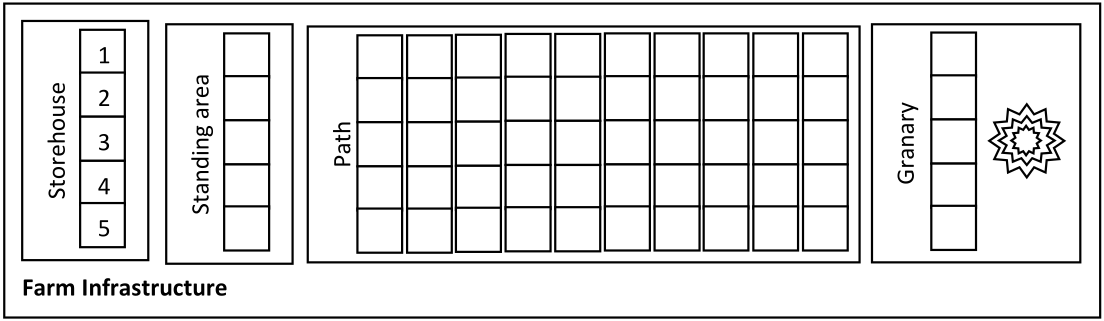
\includegraphics[width=\linewidth]{img/Design_FI.png}
%   \end{minipage}%
%   \caption{Visual representation of the farm, taken from \cite{assign}.}
%   \label{Design_FI}
% \end{figure} 

%\texttt{java -cp <userdir>/build/classes fi.FarmInfrastructure}

\newpage
\section{Scientific Computation and Custom Systems} \label{scientificcomputation} %%%%%%%%%%%%%%%%%%%%%%%%%%%%%%%%%%%%%%%%%%%%%%%%%%%%%%%%%%%%%%%%%%%%%%%%%%%%%%

Applied computer science and mathematics often use advanced computing capabilities to understand and solve complex problems.
In practical use, computational science is typically the application of computer simulation and other forms of computation to tackle problems in various
scientific disciplines.
Scientists and engineers develop computer programs that model systems being studied and run these programs with various sets of input parameters.
In some cases, these models require massive amounts of calculations and are often executed on supercomputers or distributed computing platforms.

This project does not describe one of these models, rather it is about the development of an infrastructure capable of supporting such computationally demanding tasks.
The adopted strategy was of coordinating a cluster of processing servers.
The following tactics were selected to be implemented:
\vspace{-10pt}
\begin{itemize}[noitemsep]
  \item Computation Replicas - requests must be fairly distributed amongst the servers.
  \item Concurrency - each request runs on its own thread in a server.
  \item Redundancy - in case a server goes down, requests should be reallocated.
  \item Monitor - everything must be supervised, from the cluster's status, to the clients' identification and request treatment.
  \item Horizontal scalability - new servers can be deployed whenever necessary.
\end{itemize}
\vspace{-10pt}

\subsection{The Scenario} \label{scenario} %%%%%%%%%%%%%%%%%%%%%%

In order to test the application of the infrastructure on a scientific problem, an example scenario was adopted: the calculation of the mathematical constant $\pi$ (pi).
Being an irrational number, $\pi$ cannot be expressed as a common fraction and its decimal representation never ends and never settles into a permanently repeating pattern.
Nevertheless, in the 21st century, mathematicians and computer scientists have pursued new approaches that, when combined with increasing computational power,
extended the decimal representation of $\pi$ to many trillions of digits \cite{pisky}.
The primary motivation for these computations is as a test case to develop efficient algorithms to calculate numeric series, as well as the quest to break records.

The most commonly adopted forms of calculating $\pi$ are the iterative algorithms \cite{jorg}.
In order to only focus on the infrastructure's implementation, while simulating the actual implementation of the iterative algorithms, a control variable
corresponding to the number of iterations to be used on the calculation was introduced to regulate servers' response times.

\subsection{The Messages} \label{messages} %%%%%%%%%%%%%%%%%%%%%%

One of the fundamental constraints applied to our implementation was related to communications.
Each individual server is launched as an independent process.
This is also true for each individual client.
The orchestrator runs in an independent process as well, serving as both a load balancer and a tactic monitor - although these two are built as separate entities.
So in order for entities to communicate with each other, the TCP/IP socket technology was made a requirement.

For simplicity, only two service message types were defined:
\vspace{-10pt}
\begin{itemize}[noitemsep]
  \item Request: $|$ \texttt{clientID} $|$ \texttt{requestID} $|$ \texttt{01} $|$ \texttt{\# iterations} $|$
  \item Reply: $|$ \texttt{serverID} $|$ \texttt{clientID} $|$ \texttt{requestID} $|$ \texttt{02} $|$ \texttt{\# iterations} $|$ \texttt{pi} $|$
\end{itemize}
\vspace{-10pt}
In them are the following parameters:
\texttt{clientID}, a positive integer that uniquely identifies a client machine;
\texttt{serverID}, a positive integer that uniquely identifies each physical server in the cluster;
\texttt{requestID}, a positive integer that uniquely identifies a pi calculation request (computed as 1000 $\times$ \texttt{client id} $+$ increment);
\texttt{01} and \texttt{02}, the request and reply codes;
\texttt{\# iterations}, the chosen value for the previously mentioned control variable used to simulate the number of iterations for the computation of pi
(each iteration / cycle corresponds to 1 second);
\texttt{pi}, the computed value of $\pi$.

A few additional message types were added during development for management purposes:
\vspace{-10pt}
\begin{itemize}[noitemsep]
  \item Heartbeat: ..................................
\end{itemize}
\vspace{-10pt}

..............................................................................................

\newpage
\section{System Architecture} \label{architecture} %%%%%%%%%%%%%%%%%%%%%%%%%%%%%%%%%%%%%%%%%%%%%%%%%%%%%%%%%%%%%%%%%%%%%%%%%%%%%%%%%%%%%%%%%%%%%%%%%%%%%%%%%%%%%


\subsection{Components} \label{components} %%%%%%%%%%%%%%%%%%%%%%

\subsubsection{Client}


\subsubsection{Server}


\subsubsection{Load Balancer} \label{lb}
This is one of the most important components of our architecture. It's existence started by being a project requisite, but we quickly understood and concluded that in fact it was a huge asset in our solution. This component proved to be quite paramount when handling the quality attributes we had to guarantee in this project. This component was mainly created to handle availability and scalability, reasons we will further detail in section \ref{constraints}. This section will describe how this component work.

It's main purpose, as the name implies, is to distribute in a balanced way the incoming $\pi$ calculation requests across all registered servers. When one or more calculation requests are sent to the Load Balancer, for each request the least occupied server is requested from the Tactic Manager, enabling a balanced distribution; after knowing to which server the message should be redirected to, information such as the ip and port from the client requesting the service is also requested from the Tactic Manager, allowing the server to respond to the client directly, as stated by the project guide; finally, the message is redirected to the server with the client information added in a pre-defined fashion.

Additionally, this and only this component is the one responsible for interacting with the system clients. This means that not only the already mentioned $\pi$ calculation requests but also some additional control messages that our team created need to be handled by the Load Balancer. These additional messages are related to the creation and destruction of a client. As already mentioned in section \ref{components}, we concluded and decided that the most logical approach was to enable each server to choose and define its port, due to physical restriction; this means that when a client is created, the server side of the system does not know its ip not its port, information that needs to be registered. Following that thought process, we created both a creation message, containing the client's ip and port and a deletion message containing only the client's id that was given by the Tactic Manager. Those messages in the creation or deletion of the client are sent to the Load Balancer, the only entity the client knows about in the system's server side.

When receiving the client control messages, the Balancer acknowledges it as received it and redirects the message to the Tactic Manager, that will process and store the received information, and in the case it is a client creation, it will send to that client his just created internal id.

\subsubsection{Tactic Manager}
This component can be considered as the brain of the cluster, since it should have the knowledge about every registered server, every registered client, the state and who is processing every message at anytime. This is necessary, for example,as stated in section \ref{lb}, to enable the Load Balancer to distribute in a balanced fashion the incoming calculation requests since the Manager knows the occupation of each server at anytime.

One of its responsibilities is to be the entity, and the only one, with whom the servers talk too. For that reason, similarly to the control messages developed for the clients refereed in section \ref{lb}, we also needed to create control messages for the creation and destruction of each server, being sent in the appropriate time to the Task Manager, that will process the messages and store the information, also sending the created id in case of a server creation. Additionally, all servers when receiving or finishing to process a calculation request should notify this managing entity of its status change.

Another responsibility of this component is the executions and possible consequent actions related to the health-check of all registered servers. This functionally was concluded to be paramount when assuring our quality attributes, namely Scalability, Performance, Availability and Usability. The flow of this process goes as follows: when the Tactic Manager is created, the Health-checking subprocess is initiated in parallel, and from then on, it will send a health-check to all registered servers on a time interval previously established, in our scenario it was defined at 30 seconds. In the case one server doesn't respond to the health-check, it is considered dead, and for that reason it is deleted form the internal registries and any request assigned to that server(which was previously registered by the server when alive) will be equally distributed by all remaining servers by sending them to the Load Balancer which will execute that task.

\subsection{Auxiliary Components}
%SocketServer,SocketClient,LoadDistributer, HealthChecker, AttendUser

\subsection{User Interface} \label{ui} %%%%%%%%%%%%%%%%%%%%%%%%%%


\newpage
\section{Architecture Constraints} \label{constraints} %%%%%%%%%%%%%%%%%%%%%%%%%%%%%%%%%%%%%%%%%%%%%%%%%%%%%%%%%%%%%%%%%%%%%%%%%%%%%%%%%%%%%%%%%%%%%%%%%%%%%%%%%


\subsection{Quality Attributes Assurance} \label{qaa} %%%%%%%%%%%


\subsection{User Cases Compliance} \label{compliance} %%%%%%%%%%%


\newpage
\section{Additional Remarks} \label{remarks} %%%%%%%%%%%%%%%%%%%%%%%%%%%%%%%%%%%%%%%%%%%%%%%%%%%%%%%%%%%%%%%%%%%%%%%%%%%%%%%%%%%%%%%%%%%%%%%%%%%%%%%%%%%%%%%%%%%

\subsection{Documentation} \label{documentation} %%%%%%%%%%%%%%%%

Our attitude towards the developed code was to ensure it could be applied to other similar scenarios and reused in systems intended to be deployed in real scenarios.
With this in mind, we took great care with regards to code readability.
By maintaining a code style equal throughout the project and defining intuitive and self-explaining variable and method names, we made the code easy to understand
by someone already contextualized with Kafka.

Nevertheless, we wanted to make sure this was also true to someone looking at our project for the first time, so we resorted to the well-known Javadoc
\cite{javadoc} tool to manage all code documentation.
Comments were also added in key points throughout the code, including the scripts.

\subsection{Assignment Contributions} \label{contributions} %%%%%

As the entire development phase took place in a time where on-site cooperation was not possible, we resorted to online communication platforms to debate decisions
and discuss difficulties.
Team scheduling allowed us to work on the project simultaneously, so no member suffered from unbalanced workloads.
The dimension of the project did not appeal to the usage of repository pull requests and other synchronization tools.
However, each small solution was verified and agreed by both team members.

Having said this, it is difficult to isolate what each member actually implemented, as the influence of both is present in all components.
Nevertheless, one might say that each had stronger responsibilities on a set of project aspects:
Filipe took care of the execution of the individual Java processes and of the Shell scripts, while João developed the Kafka-related classes such as Consumer,
Producer and EntityAction; Filipe developed the Python script for generation of \texttt{CAR.TXT}, while João developed the Shell scripts for Kafka initialization
and deletion; each implemented 2 entities and each wrote a portion of this report; Filipe made sure everything was coherent throughout the report and the code
documentation, while João solved the most critical issues regarding the configuration of the topics.
In terms of work percentage, we believe it was about 50\% for each student.

\newpage
\section*{Conclusions} \label{conclusions} %%%%%%%%%%%%%%%%%%%%%%%%%%%%%%%%%%%%%%%%%%%%%%%%%%%%%%%%%%%%%%%%%%%%%%%%%%%%%%%%%%%%%%%%%%%%%%%%%%%%%%%%%%%%%%%%%%%%%

\begin{thebibliography}{9} %%%%%%%%%%%%%%%%%%%%%%%%%%%%%%%%%%%%%%%%%%%%%%%%%%%%%%%%%%%%%%%%%%%%%%%%%%%%%%%%%%%%%%%%%%%%%%%%%%%%%%%%%%%%%%%%%%%%%%%%%%%%%%%%%%%%%
  \bibliographystyle{Science}

  \bibitem{pisky}
  \textit{Pi in the sky: Calculating a record-breaking 31.4 trillion digits of Archimedes' constant on Google Cloud}.
  Taken from \href{https://web.archive.org/web/20191019023120/https://cloud.google.com/blog/products/compute/calculating-31-4-trillion-digits-of-archimedes-constant-on-google-cloud}{web.archive.org}.
  Retrieved May 2020.

  \bibitem{jorg}
  Arndt, Jorg \& Haenel, Christoph (2006).
  \textit{Pi Unleashed}, in Springer-Verlag.
  ISBN 978-3-540-66572-4.
  Retrieved May 2020.
  English translation by Catriona and David Lischka.

  % \bibitem{uml}
  %   Object Management Group,
  %   \textit{What is UML},
  %   \url{https://www.uml.org/what-is-uml.htm},
  %   accessed in March 2020.

\end{thebibliography}

\clearpage

\end{document}




















